\documentclass[a4paper,11.5pt]{article}
\usepackage[latin1]{inputenc}
\usepackage[T1]{fontenc}
\usepackage[english]{babel}
\usepackage{graphicx}
\usepackage{amsmath}
\usepackage{amsfonts}
\usepackage{multirow}
\usepackage{booktabs}

\newcommand{\eq}{\begin{equation}}
\newcommand{\feq}{\end{equation}}
\newcommand{\vt}{\boldsymbol}
\newcommand{\itz}{\begin{itemize}}
\newcommand{\fitz}{\end{itemize}}

\title{Digital Communications - HW2}
\author{Jacopo Pegoraro, Edoardo Vanin}
\date{24/04/2018}

\begin{document}

\maketitle

\section*{Exercise 1}

We want to estimate the impulse response of an IIR real system affected by white noise and with different sampling period between the input and the output, putting ourselves at the receiver so knowing only the output of the system, the input and a bound on the order of the system (approximating the IIR with an FIR). In particular we call the input of the system $x(kT_x)$ with $T_x=1$, that undergoes upsampling of a factor 2 becoming $y(mT_y)$ with $T_y=\frac{T_x}{2}$ and is then filtered with an impulse response $h$ defined on $T_y$ that is what we want to estimate. To the output of the filter $z(mT_y)$ is added a white gaussian noise $w(mT_y)$ with variance $\sigma_w^2=-8$ dB. We call the overall output after all these operations $r(mT_y)$. The difference equation of the filter is known at the transmitter and is, neglecting the dependance on $T_y$ for an easier notation:
\begin{equation} \label{eq:diff}
z(m)=-a_1z(m-1)-a_2z(m-2)+y(m)
\end{equation}
\noindent where $a_1=-0.9635$ and $a_2=0.4642$. 
To do the estimation we need to use as input a PN sequence and approximate the IIR filter with an FIR of order $N_h\le20$. However, we only know methods that can work if the input and the output of the filter are defined on the same sampling period, while in this case $h$ is defined on $T_y$. To solve the problem we exploit the polyphase representation of the system, dividing $h$ in $h^{(0)}$ and $h^{(1)}$ that act respectively only on the even and odd samples of the input (we are using the \emph{first noble identity} to transform the cascade of the upsampler and the filter in the separate filtering by $h^{(0)}$ and $h^{(1)}$ followed by a parallel to serial converter \cite{nevio<3}). Once the equivalent system is derived, we can perform separately the estimates of $h^{(0)}$ and $h^{(1)}$ that are now defined on the same sampling time as their input ($T_x$). Two different methods will be used on both the polyphase components: the correlation method and the least squares method (LS) \cite{nevio<3}. In the following sections we give a brief description of the structure of the PN sequences and of the two methods.

\subsection*{PN sequences}

PN sequences are deterministic and periodic binary sequences that, despite their non-random nature, present characteristics that make them suitable to simulate a white noise while being much more simple to generate \cite{nevio<3}. In this work we will use a type of PN sequences called Maximal Length sequences (ML) that can be obtained with recursive equations and the use of a shift register and the xor operator. ML sequences are defined giving their length $L$ that has to be an integer that precedes a power of 2 (here we will use sequences of length 7, 15, 31, 63, 127, 255). They can be generated starting with an arbitrary binary vector of length $r$ (where $r$ is the integer that satisfies $2^r -1=L$) and applying a difference equation that changes for every $L$ (we do not report her all the equations used and we refer to \cite{nevio<3}). The initial vector must not be the zero vector.
To estimate the channel we will use a ML sequence repeated 2 times to be able to eliminate the transient on the output when we need to, without computing the exact number of samples affected by transient behavior. The correlation and the mean of a ML sequence (using $-1$ and $1$ as binary values to eliminate biases) are:
$$
mean=\frac{1}{L}
$$
$$
r_{ML}=\begin{cases} 1 & \mbox{for  }  (n)_{modL} =0 \\
-\frac{1}{L} & \mbox{otherwise} \end{cases}
$$
\noindent that get closer to the ones of a white noise as $L$ increases. It's important to recall that to have good results in channel estimation using as input ML sequences we need to stick to the situation where $L$ is much bigger than $N$, otherwise the fact that mean and variance are not the same as a white noise will become more and more influent and affect the results.

\subsection*{Correlation method}

The correlation method is based on the schema represented in figure \ref{fig:systID}, but in our analysis we used $r(k)$ instead of $d(k)$ to be consistent with the notation.  

\begin{figure}[ht]
	\begin{center}    
		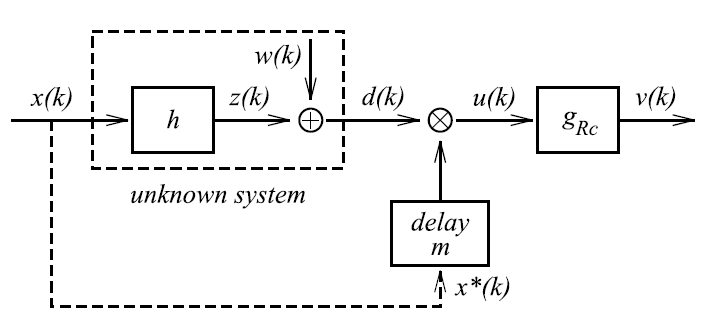
\includegraphics[width=10cm]{figs/systemID.png}
		\caption{Schema of the correlation method.}
		\label{fig:systID}
	\end{center}
\end{figure} 

\noindent The impulse response to be estimated is approximately equal to the correlation between the input sequence and the output of the unknown system (after the addition of the noise). I formulas:
\begin{equation} \label{eq:corr}
\hat{r}_{rx}(m)= \frac{1}{L} \sum_{k=L-1}^{2L-2}r(k)p^*(k-m)
\end{equation}
\noindent where we use the samples od $d(k)$ starting from $L-1$ to be sure we skip the transient. To adapt this procedure to our specific case we computed the output of the real system using the difference equation (\ref{eq:diff}). Dividing the output $r(m)$ in its even/odd samples $r^{(0)}$ and $r^{(1)}$ we obtained the target output of the polyphase components $h^{(0)}$ and $h^{(1)}$ to be used in \ref{eq:corr}. For each component then we carried out the computation of the correlation. The result is an estimate of the polyphase components from which we built the estimate $\hat{h}_{corr}$ of the complete impulse response by arranging the coefficients of the components as even and odd coefficients of $\hat{h}_{corr}$. As a measure of the error we make in estimating the coefficients we used the same functional as in the LS method (see the next section): $\mathcal{E}_{corr} = \sum_{k=L-1}^{2L-2}|r(k)-\hat{r}(k)|^2$, where $\hat{r}(k)$ is the output computed using the estimated impulse response. An estimate of the noise variance can be obtained with $\hat{\sigma}_{w,corr}^2=\frac{1}{L}\mathcal{E}_{corr} $.

\subsection*{LS method}

The LS method aims to minimize the functional $\mathcal{E} = \sum_{k=L-1}^{2L-2}|r(k)-\hat{r}(k)|^2$ where the expressions of the target output and the estimated output are:
\begin{equation}
r(k)=\vt{h}^T\vt{x}(k)+w(k)
\end{equation}
\begin{equation}
\hat{r}(k)=\hat{\vt{h}}^T\vt{x}(k)
\end{equation}
\noindent and we introduce the matrix $\vt{\Phi}$ and the vector $\vt{\theta}$:

\begin{equation}
\Phi (i,n)=\sum_{k=L-1}^{2L-2}x^*(k-i)x(k-n)
\end{equation}

\begin{equation}
\theta (n)=\sum_{k=L-1}^{2L-2}r(k)x^*(k-n)
\end{equation}
\noindent that have, respectively, dimensions $(L-1)\times(L-1)$ and $(L-1)\times 1$. To simplify the computation of the two quantities we introduce the data matrix $\boldsymbol{\mathcal{I}}$, defined as:

\begin{equation}
\vt{\mathcal{I}} =
\begin{bmatrix}
x(L-1)	& \cdots &	x(0) \\
\vdots	& \vdots & \vdots \\
x(2L-2)	& \cdots &	x(L-1)
\end{bmatrix}
\end{equation}
\noindent and the desired sample vector:
\begin{equation}
\vt{o}^T=[r(L-1) \ \ \ r(L-2) \ \ \  \dots \ \ \ r(2L-2)]
\end{equation}
\noindent from which we can obtain $\vt{\Phi}$ and $\vt{\theta}$ as  $\vt{\Phi}=\vt{\mathcal{I}}^H\vt{\mathcal{I}}$, $\vt{\theta}=\vt{\mathcal{I}}^H\vt{o}$. 
The solution of the LS estimate is given by $\hat{\vt{h}}_{ls}=\vt{\Phi}^{-1}\vt{\theta}$. An estimate of the noise variance can be obtained with $\hat{\sigma}_{w,ls}^2=\frac{1}{L}\mathcal{E}_{ls} $ where $\mathcal{E}_{ls}$ is the mean squared error functional computed with the output obtained by filtering $x(k)$ with $\hat{h}_{ls}$.

As with the correlation method, here too the estimate is done separately for the 2 polyphase components by dividing the even and odd samples of the output signal $r(m)$.


\subsection*{Numerical Results}

\begin{figure}[ht]
	\begin{center}    
		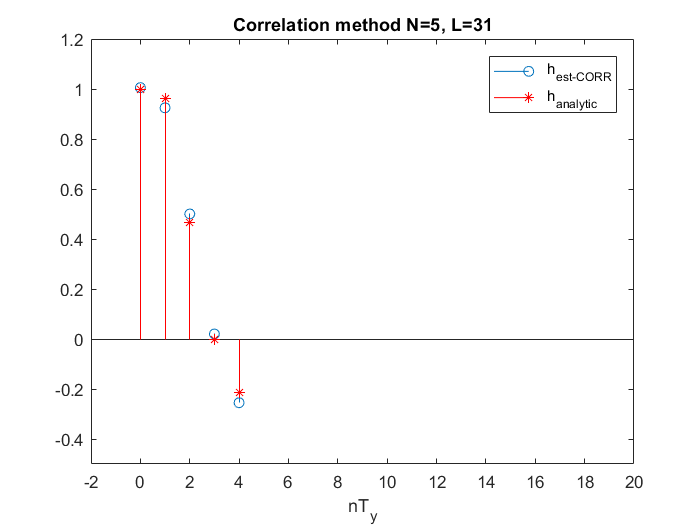
\includegraphics[width=6cm]{figs/corrN5L31.png}
		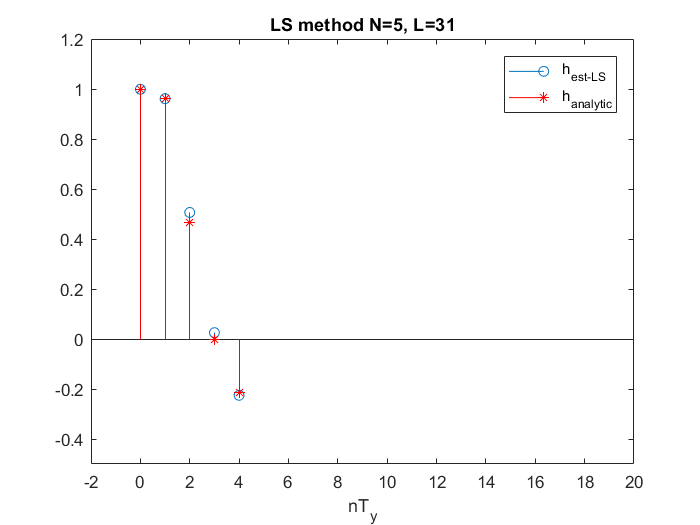
\includegraphics[width=6cm]{figs/lsN5L31.png}
		\caption{$h$ and $\hat{h}$ with the correlation and LS method for the final choice of the parameters L=31 and N=5 .}
		\label{fig:hest}
	\end{center}
\end{figure} 
 
 \begin{figure}[ht]
 	\begin{center}    
 		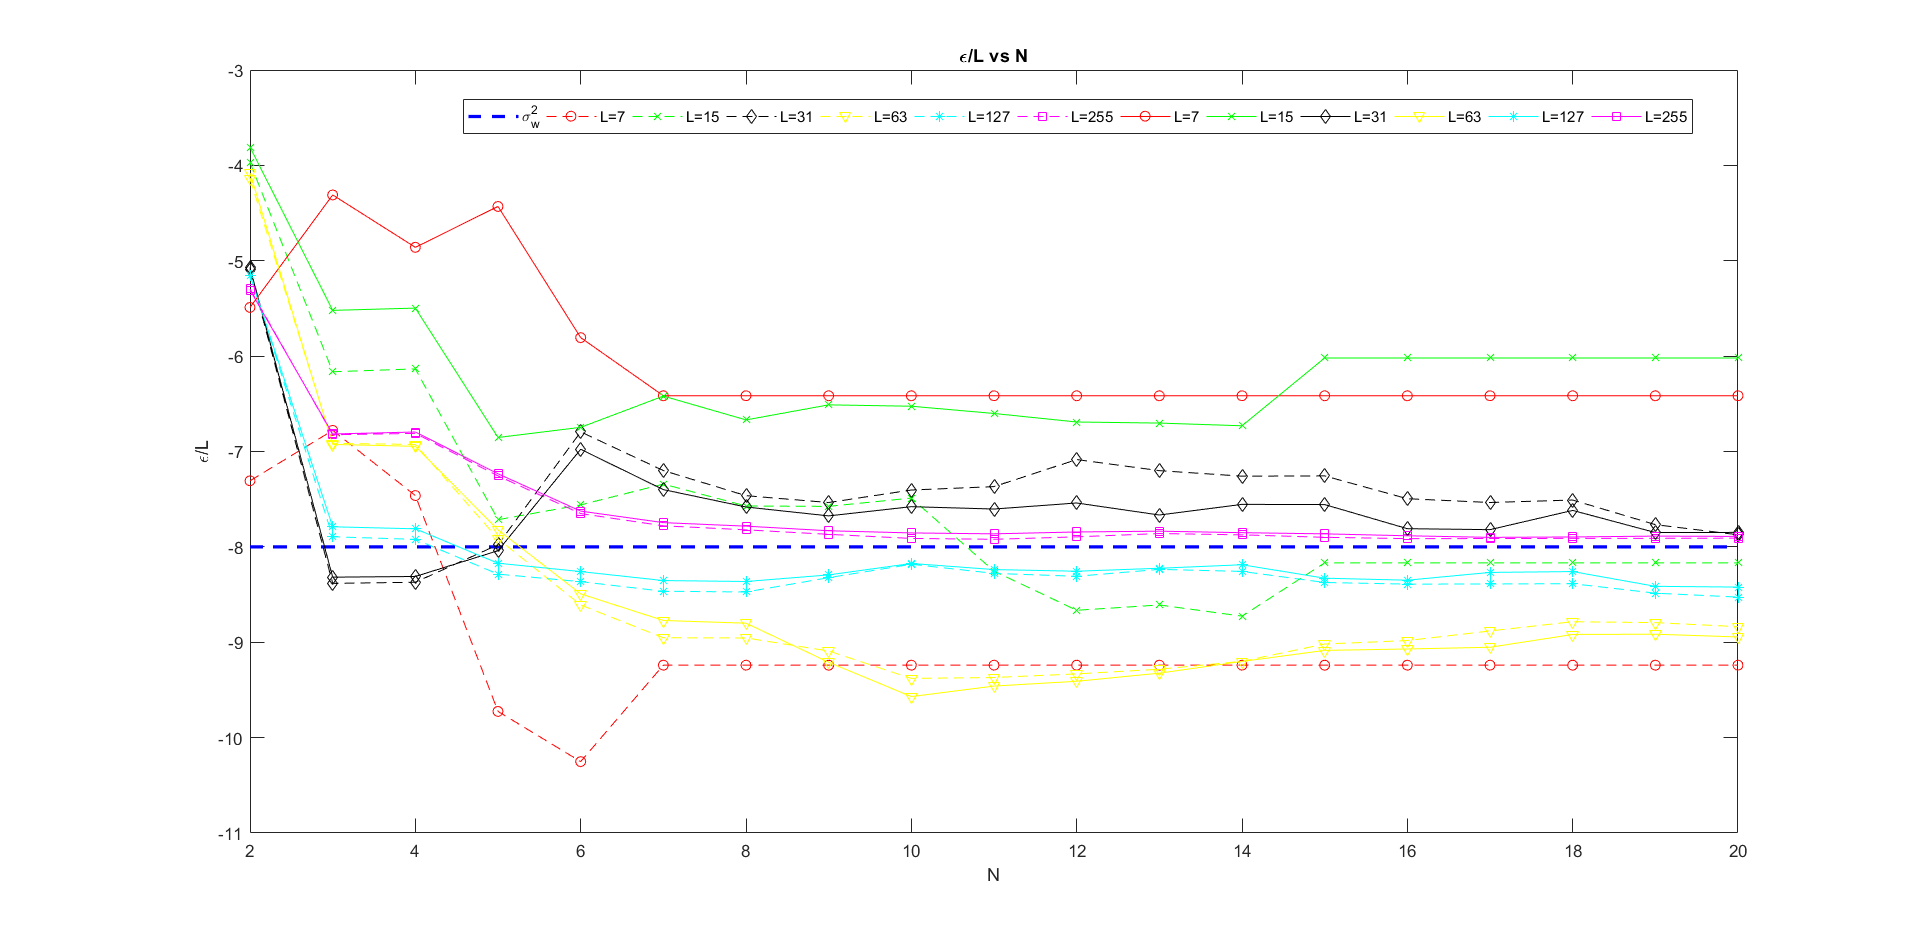
\includegraphics[width=\textwidth]{figs/L-N-choice.png}
 		\caption{Plot of the estimated variance of the noise varying L and N.}
 		\label{fig:L-N}
 	\end{center}
 \end{figure} 

\section*{Exercise 2}
\begin{figure}[ht]
	\begin{center}    
		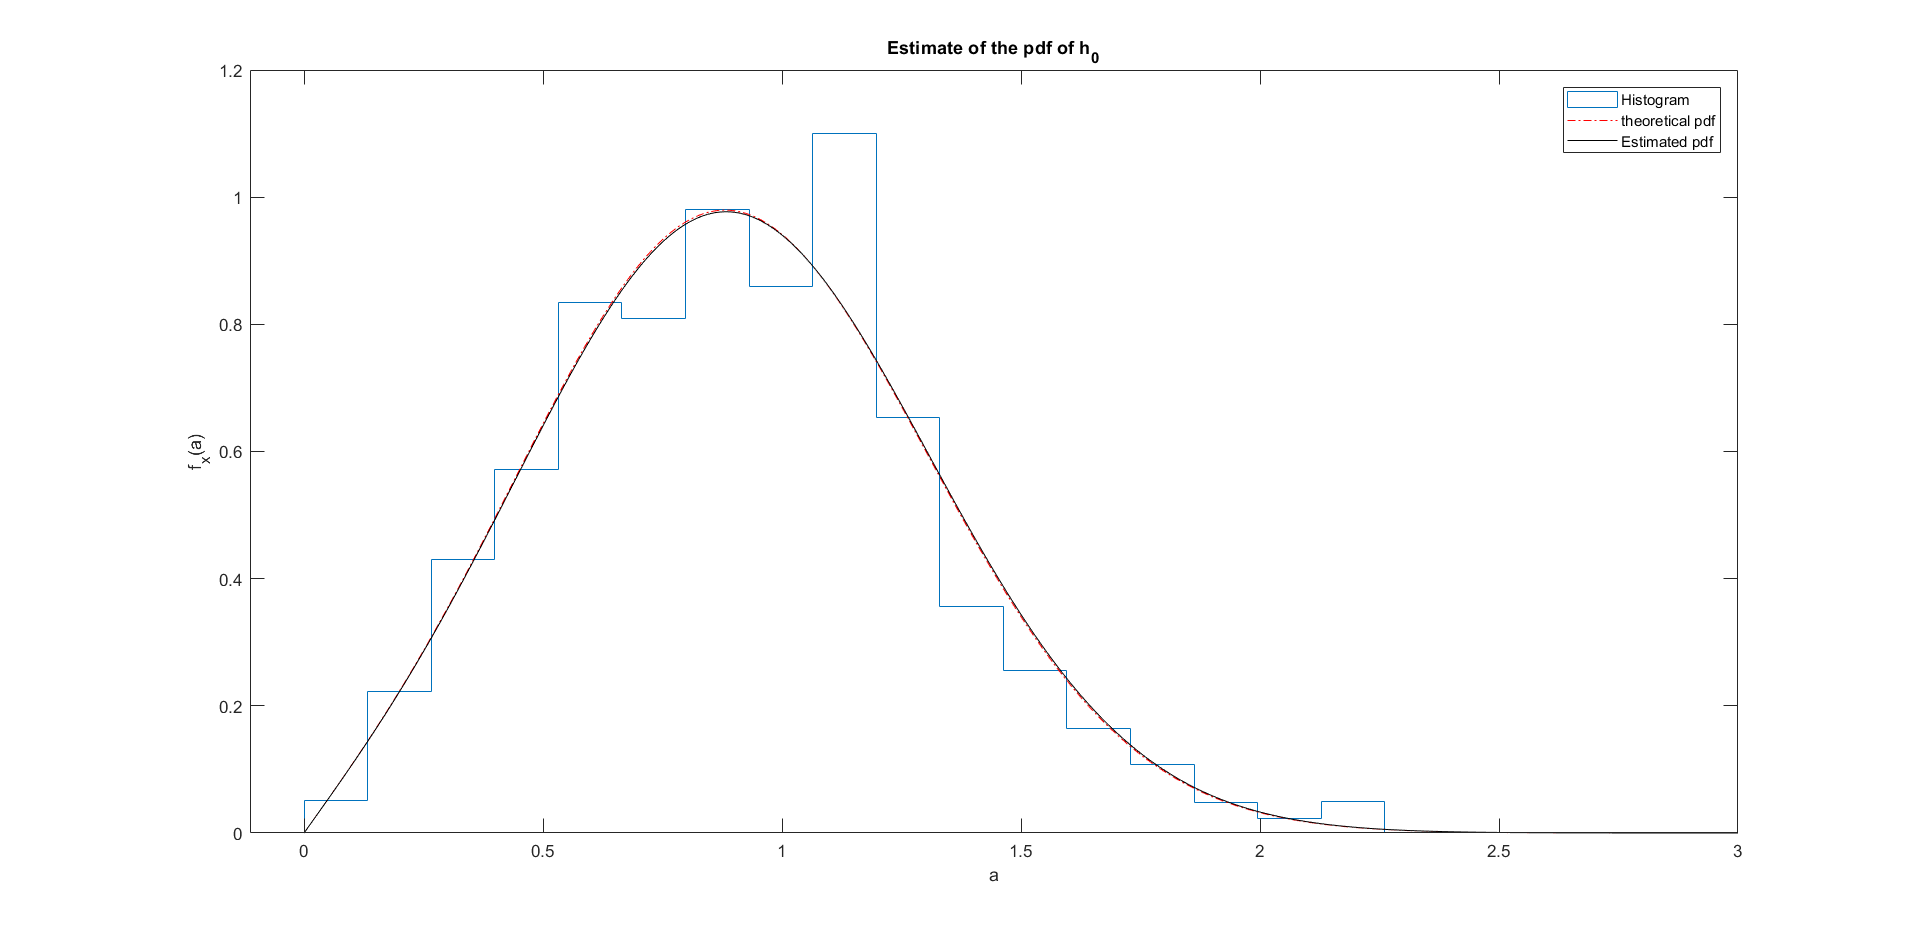
\includegraphics[width=\textwidth]{figs/estimate-pdf.png}
		\caption{Estimate of the pdf of $|h_0|$ by an histogram.}
		\label{fig:hist}
	\end{center}
\end{figure} 

\begin{thebibliography}{15}
	\bibitem{nevio<3}
	Nevio Benvenuto, Giovanni Cherubini,
	\textit{Algorithms for Communication Systems and their Applications}. 
	Wiley, 2002.
\end{thebibliography}

\end{document}